\section{Challenges en ergonomie}

\subsection{Implémentations réalisées et structure du front-end}

Le principal but en matière d'ergonomie a été de \textbf{fournir une interface} au plugin "interactif" de Psyche. Pour parvenir à l'interface présentée en figure \ref{interface_global}, les difficultés relèvent surtout de l'implémentation et de la communication avec le noyau de Psyche.

\begin{figure}[!ht]
    \center
    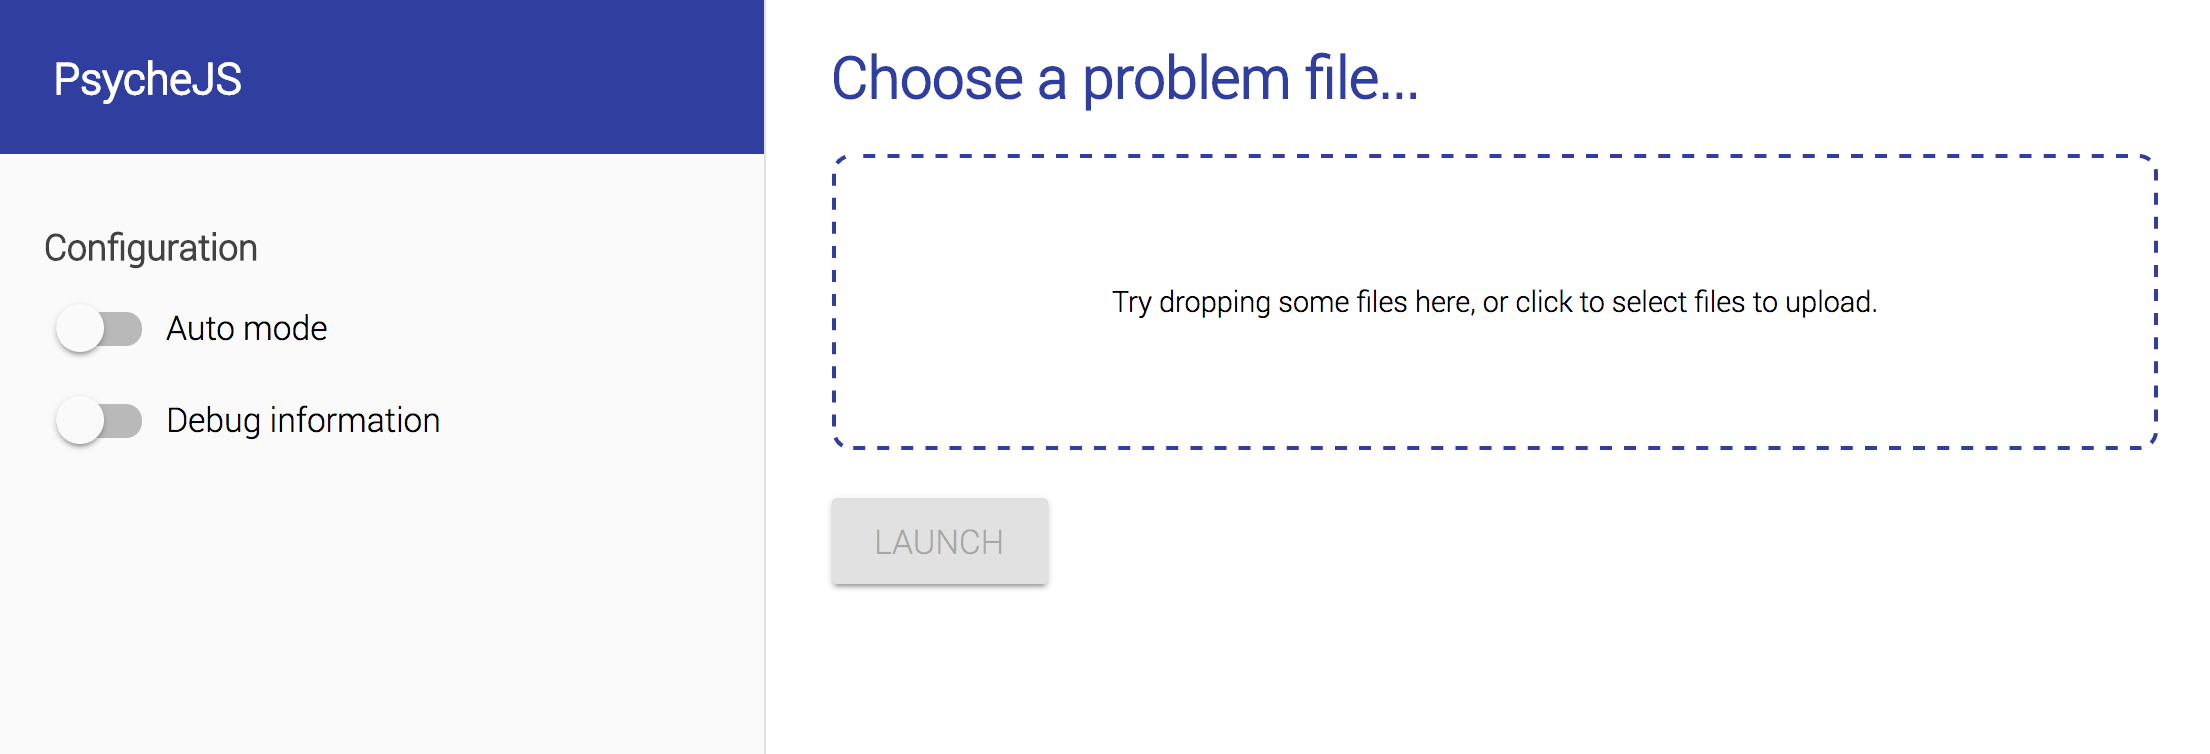
\includegraphics[width=1\textwidth]{./images/III_1_interface_1.png}
    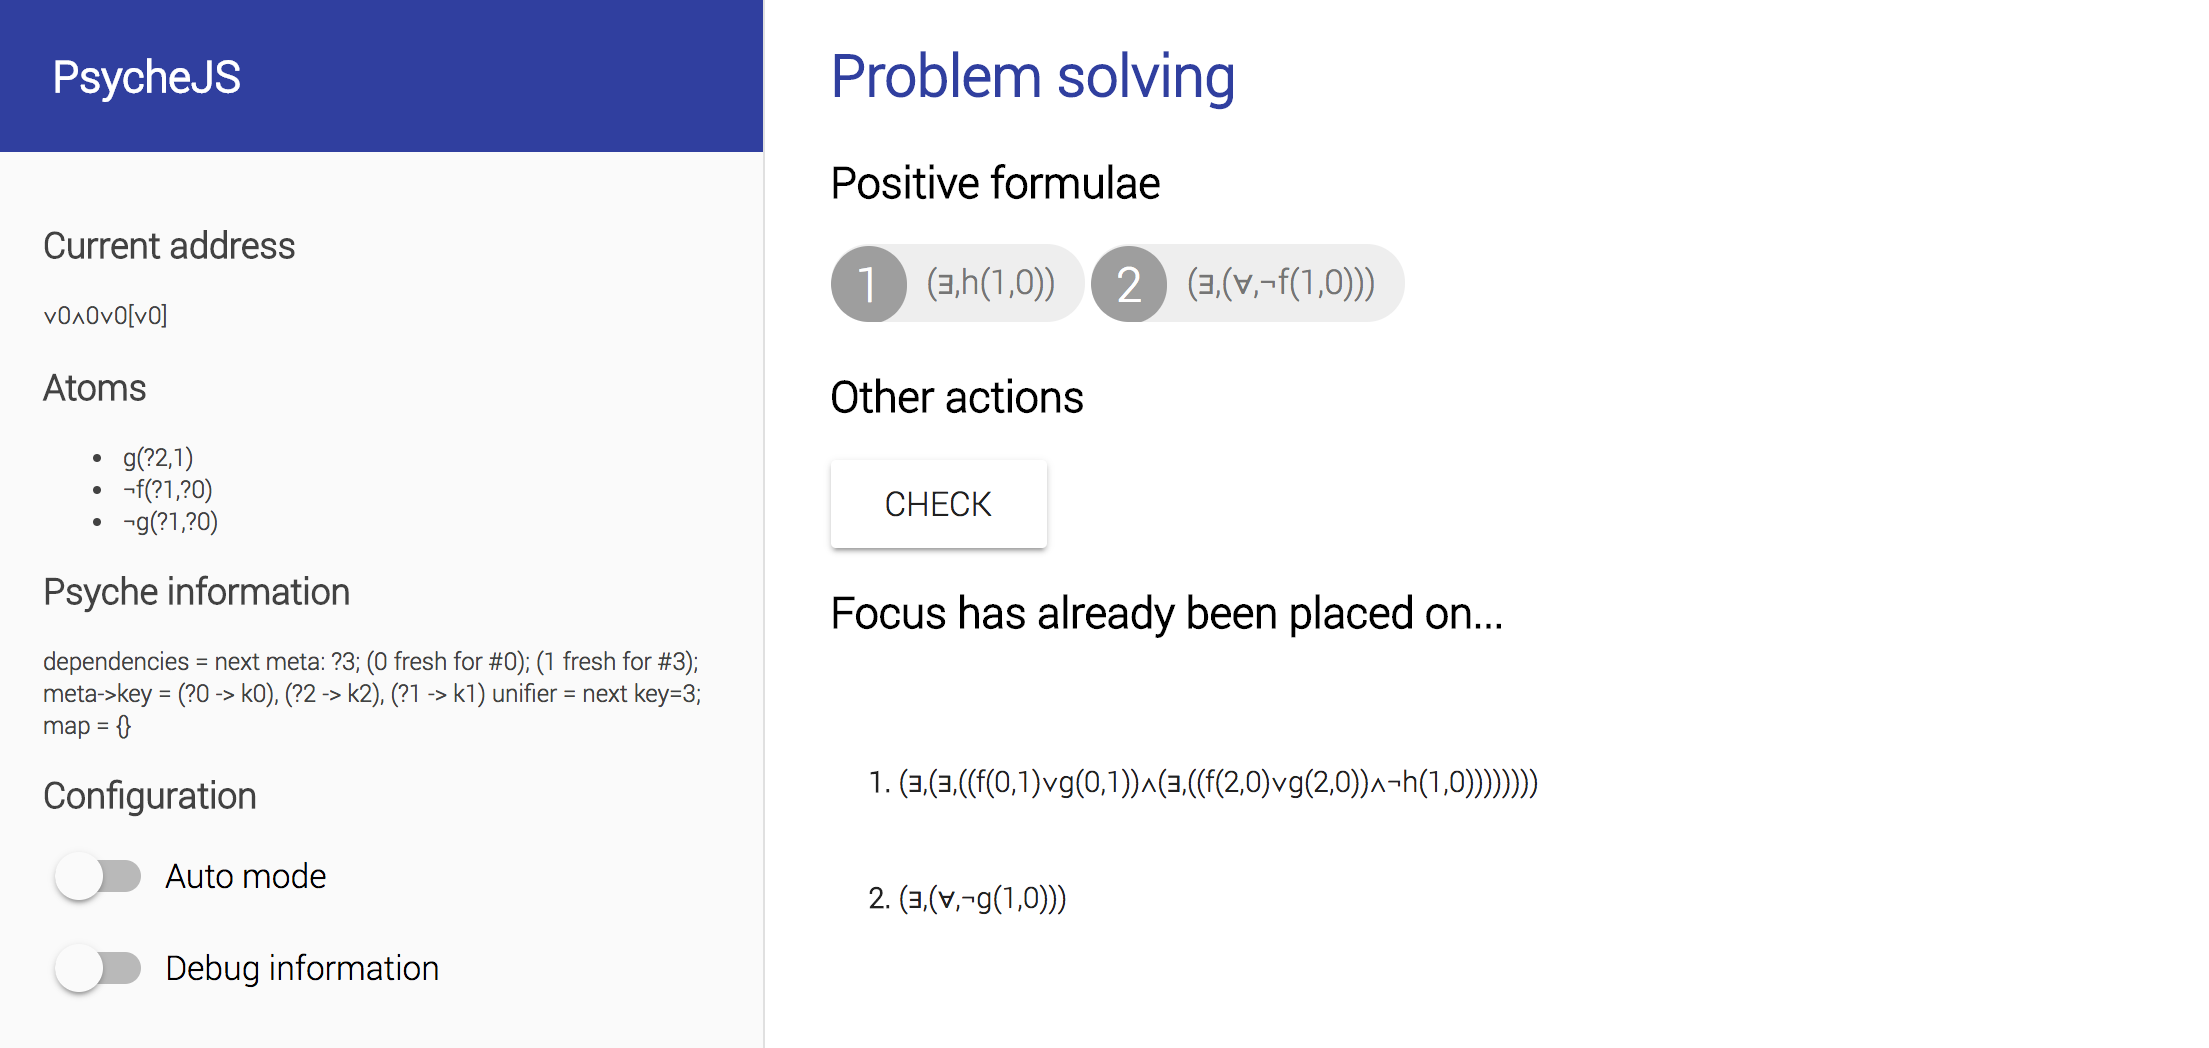
\includegraphics[width=1\textwidth]{./images/III_1_interface_2.png}
    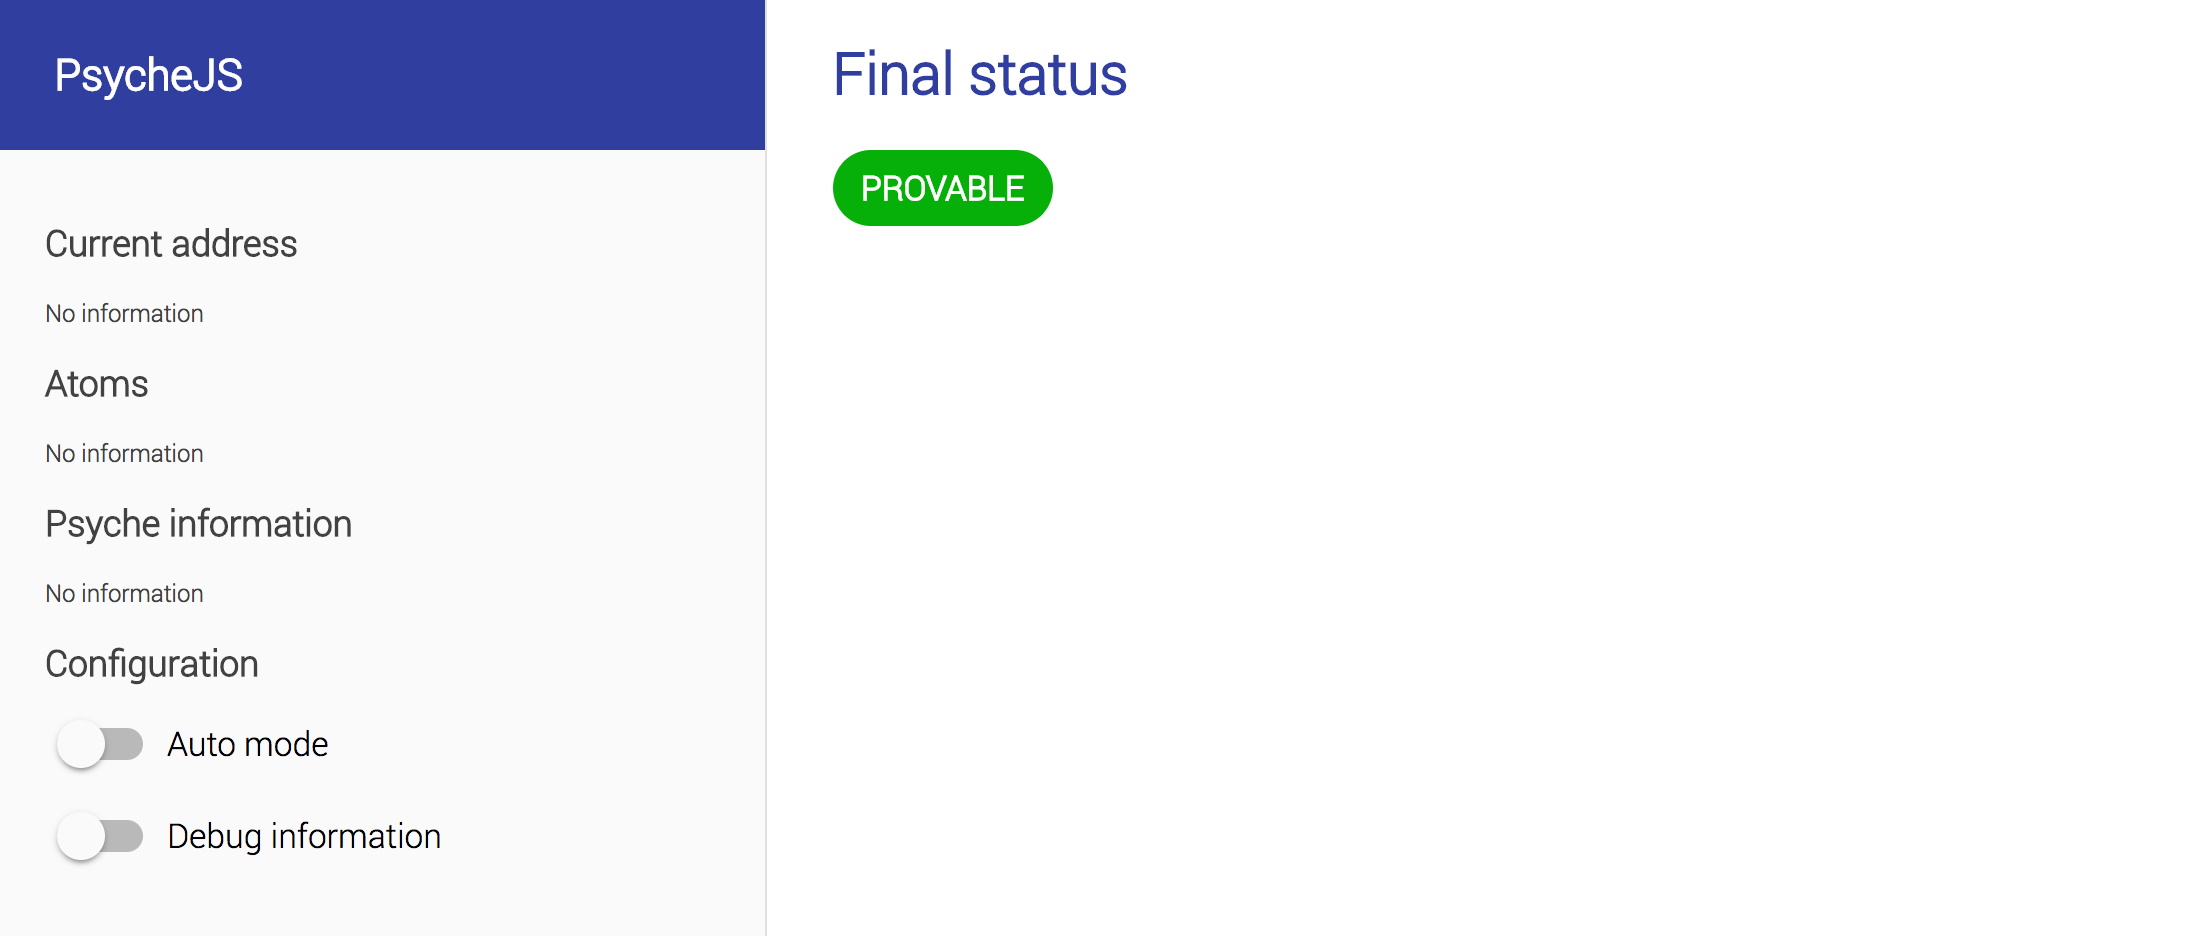
\includegraphics[width=1\textwidth]{./images/III_1_interface_3.png}
    \caption{\label{interface_global} L'interface actuelle de l'outil développé.}
\end{figure}

En premier lieu, l'utilisateur charge le fichier décrivant le problème à traiter -- au même format que celui accepté par Psyche --, qui est ensuite fourni au noyau. Si l'utilisateur reste en mode interactif, l'interface lui demande à chaque fois que le noyau de Psyche lui rend la main quelle action prendre, parmi :

\begin{itemize}
\item Choisir une formule sur laquelle placer le focus parmi les formules disponibles ;
\item Tenter d'unifier les contraintes courantes en faisant un "check".
\end{itemize}

Pour l'aider dans son choix, l'interface lui donne des informations fournies par Psyche, comme l'adresse courante dans l'espace de recherche ainsi que les formules sur laquelle le focus a déjà été placé.\\

L'utilisateur peut également tenter de laisser l'interface décider pour lui en activant l'option "Auto mode". L'interface inclut en effet une implémentation d'un plugin naïf de Psyche, mais qui ne fonctionne que sur quelques problèmes très simples\footnote{Il se trouve que la dernière version de Psyche embarque un plugin "naïf" beaucoup plus performant et qui peut résoudre des problèmes plus compliqués}.\\

L'interface s'appuie largement sur les composants graphiques proposés par la librairie \textbf{React Toolbox}\footnote{Voir : \url{http://react-toolbox.com/}}, qui implémente les spécifications de design de Material Design, et est organisée en plusieurs composants. Selon la philosophiie de ReactJS, chaque partie indépendante de l'interface est encapsulée dans un \textbf{composant} qui a ses propres propriétés, ses propres fonctions, son propre état et son propre rendu. Pour illustrer cela, prenons l'exemple du fichier \texttt{App.js} qui est le composant global de l'application :

\begin{minted}{js}
import React, { Component } from 'react';
import './App.css';
import { init } from './dataflow/initState.js';
//import { parser } from './modules/inputParser.js';

// Components imports
import AppBar from 'react-toolbox/lib/app_bar';
import { Layout, NavDrawer, Panel } from 'react-toolbox';

// Presentational components imports
import LeftPanel from './components/presentational/LeftPanel';

// Container components imports
import TopPanelContainer from './components/containers/TopPanelContainer';

class App extends Component {
  constructor(props) {
    super(props);
    init();
  }

  render() {
    return (
      <div className="App">
        <Layout>
          <NavDrawer active={true} pinned={true}>
            <AppBar title="PsycheJS"></AppBar>
            <LeftPanel />
          </NavDrawer>
          <Panel>
            <div className="MainPanelContainer">
              <TopPanelContainer />
            </div>
          </Panel>
        </Layout>
      </div>
    );
  }
}

export default App;
\end{minted}

Le fichier commence par des imports de composants et de librairies. On définit ensuite un composant donc le constructeur ne fait rien d'autre qu'appeler une fonction \texttt{init()} définie ailleurs. Chaque composant a nécessairement une méthode \texttt{render()} qui renvoie le contenu du composant dans un langage balisé, proche du HTML et spécifique à React. Ce langage permet de définir des éléments HTML classiques, mais également de rajouter des composants React en leur passant des \textbf{propriétés} choisies. Le composant \texttt{AppBar} est par exemple fourni par la librairie React Toolbox et attend que l'on précise via ses propriétés le titre à afficher dans l'interface -- comme on l'observe sur la figure \ref{interface_global}. Le moteur React se charge ensuite de générer dynamiquement du code HTML vailde à afficher dans le navigateur.\\

En théorie, il est parfaitement possible de mettre l'état complet de l'application dans un composant global, de passer les informations nécessaires aux sous-composants via leurs propriétés et de laisser les sous-composants modifier l'état global de l'application en leur fournissant des \textit{setters} qui leur permettent de modifier l'état du composant global. En pratique, cela devient très vite ingérable, même sur des projets de petite taille, et rend le \textbf{code difficilement maintenable} : il devient vite coûteux de fournir à un composant hiérarchiquement éloigné du composant global une simple information issue de l'état de l'application.\\

Pour remédier à ces difficultés, l'application utilise la librairie \textbf{Redux}, qui fournit un état global à l'application et une manière de gérer de manière fluide les flux de données entre composants. Redux facilite notamment grandement la communication entre composants et les appels asynchrones\footnote{Les appels asynchrones sont gérés dans l'application grâce à des \textit{"promesses"} Javascript. Plus d'informations sur les objets \texttt{Promise} sont disponibles ici : \url{https://developer.mozilla.org/fr/docs/Web/JavaScript/Reference/Objets_globaux/Promise}.} au noyau de Psyche. L'article \cite{redux2016} permet de comprendre les bases du fonctionnement de Redux.

\subsection{Propositions d'évolutions}

Le projet a également été l'occasion de réfléchir à des améliorations possibles de l'interface développée. Ces propositions n'ont pas pu être implémentées pendant le développement du projet, mais ce sont des \textbf{hypothèses à tester}.\\

La première fonctionnalité est de permettre à l'utilisateur d'avoir une \textbf{vision globale de l'arbre de recherche} en cours d'exploration, et surtout d'offrir la possibilité de \textbf{défaire des actions} et de revenir à un état précédent de la preuve. La possibilité de revenir en arrière est donnée par des IDE comme \textit{Proof General}, mais sans qu'elle ne soit accompagnée d'un moyen visuel de se repérer dans l'état de la preuve. La preuve interactive de théorèmes se faisant par une méthode très exploratoire, il paraît important de pouvoir se déplacer comme on le souhaite parmi les différents états de la preuve. Offrir une vision de l'espace de recherche qui soit lisible reste toutefois un défi quand on envisage des arbres de recherche de grande taille.\\

Les autres améliorations possibles tournent autour de l'idée d'un \textbf{champ de saisie unique et multifonctions} dans l'interface. Le constat est d'une part qu'il est souvent plus pratique pour beaucoup d'utilisateurs de pouvoir tout effectuer au clavier sans avoir à utiliser la souris pour sélectionner des formules, et d'autre part qu'il faut pouvoir permettre à l'utilisateur de saisir lui-même des formules, par exemple pour effectuer des coupures.\\

En ce qui concerne l'utilisation complète de l'interface au clavier, cela passerait par des raccourcis simples et actifs même en-dehors du champ de saisie envisagé. On pourrait par exemple penser à utiliser des raccourcis classiques pour défaire et refaire des actions -- les usuels \texttt{Ctrl + Z} et \texttt{Ctrl + Maj + Z} --, à effectuer un check lorsque l'utilisateur appuie sur \texttt{Ctrl + Entrée} et à mettre le focus sur la formule numéro \texttt{i} lorsque l'interface capture la combinaison \texttt{Ctrl + i}. Evidemment, l'utilisabilité des raccourcis proposés doit être testée et il est possible que d'autres combinaisons soient optimales en termes de confort d'utilisation.\\

On peut envisager qu'une autre combinison dédiée fasse apparaître le champ de saisie dans un cadre flottant -- à la manière de l'outil de recherche Spotlight développé par Apple, qui fait apparaître un champ flottant et des suggestions de résultats en dessous, comme sur la figure \ref{spotlight}.

\begin{figure}[!ht]
    \center
    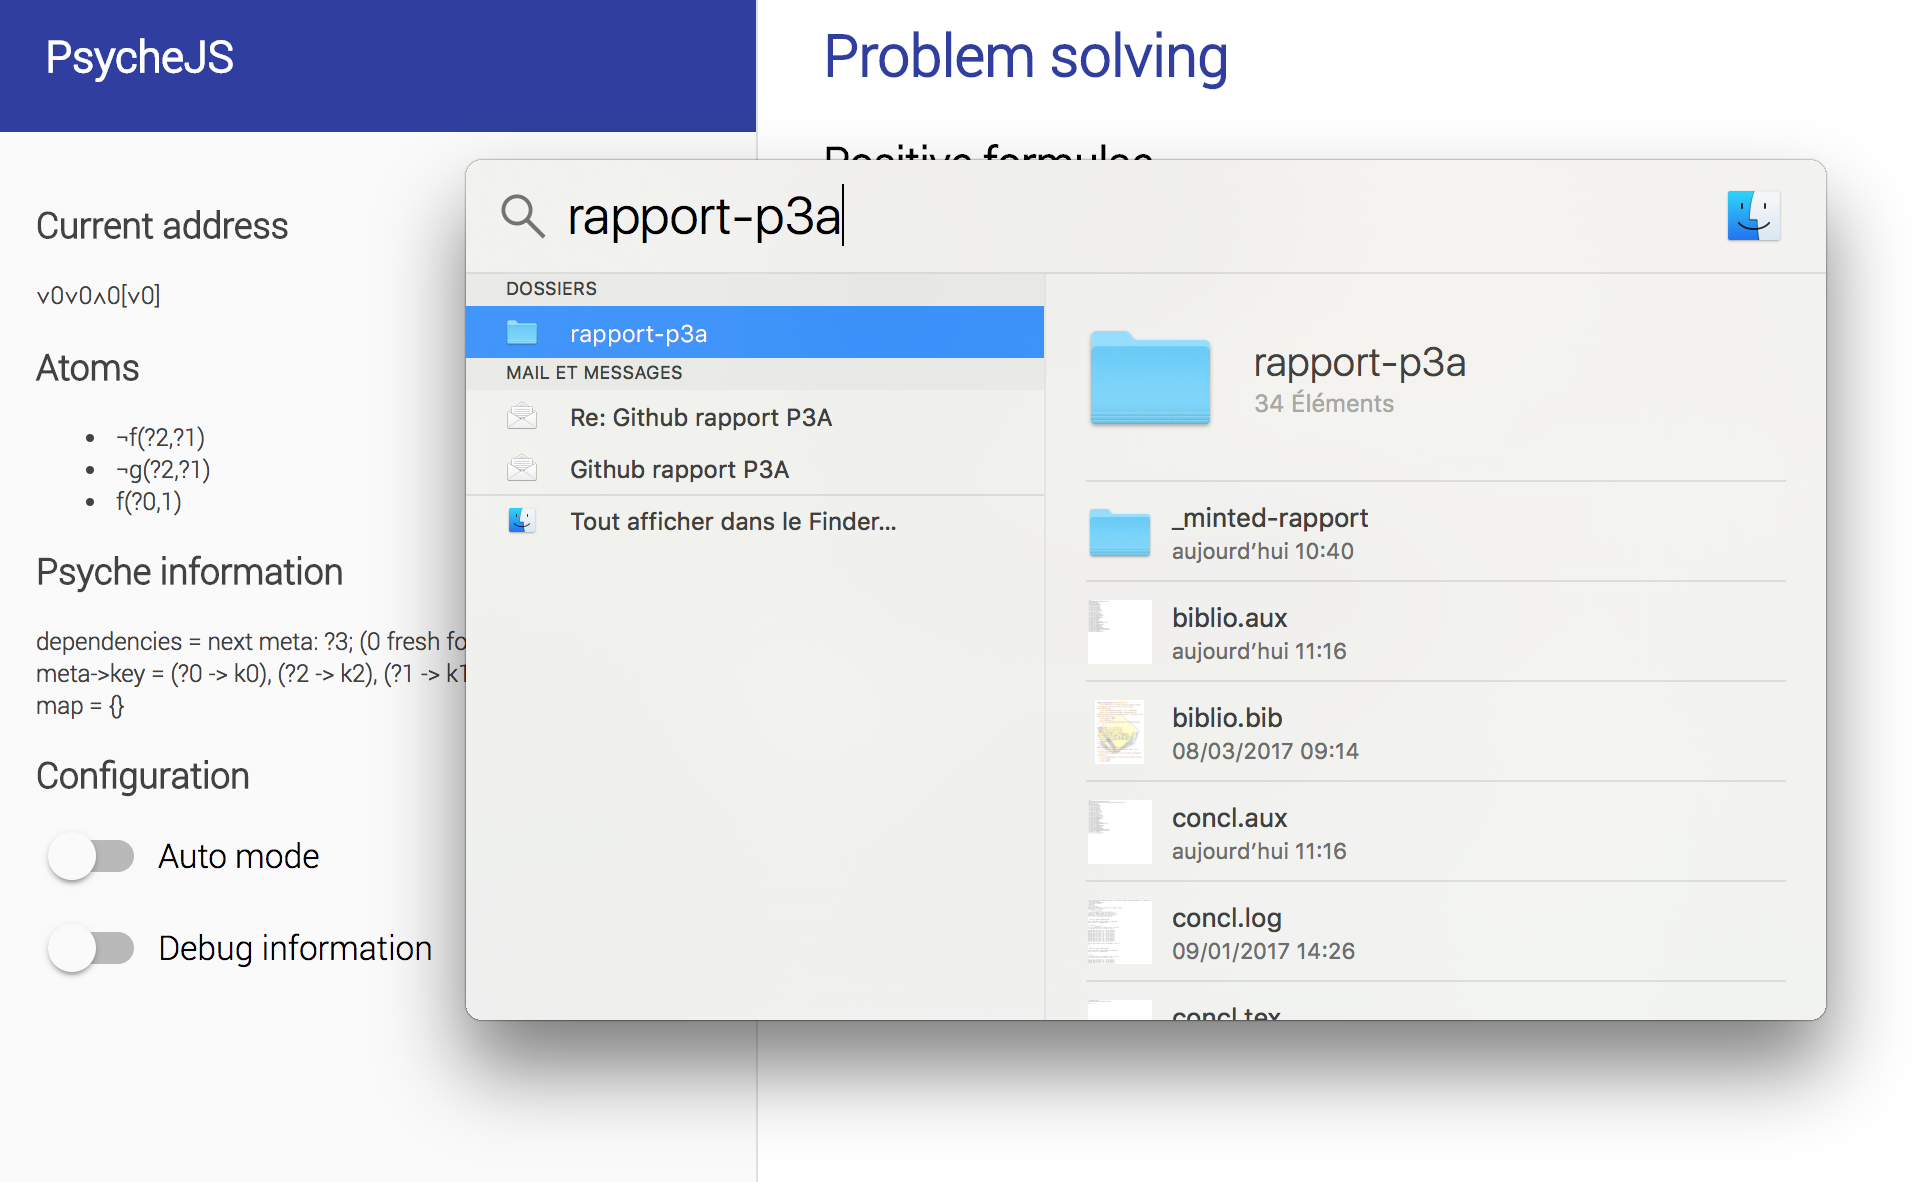
\includegraphics[width=1\textwidth]{./images/III_2_spotlight.png}
    \caption{\label{spotlight} La barre de recherche Spotlight comme inspiration ?}
\end{figure}

L'idée serait de pouvoir saisir des instructions et des formules dans un \textbf{langage naturel} et d'utiliser un lexeur et un parseur pour les rendre utilisables par l'application. La saisie suivante, par exemple

\begin{verbatim}
cut exists 1 and (not 0 or 1)
\end{verbatim}

pourrait permettre d'effectuer une coupure en utilisant une formule semblable à $\exists y, y \wedge (\bar{x} \vee y)$. Une zone de suggestions pourrait même permettre de \textbf{proposer à l'utilisateur des formules} "proches" de celle qu'il a commencée à taper et qui apparaissent dans le problème. Les fonctionnalités de cette zone de saisie pourraient être étendues à la sauvegarde et la réutilisation de sous-formules que l'utilisateur a tapé. Il peut en effet arriver que l'on veuille sauvegarder une formule pour un usage ultérieur, ou repartir d'une formule existante pour en construire une autre.\\

Beaucoup de ces hypothèses représentent un défi intéressant et complexe en termes d'implémentation. On peut par exemple raisonnablement penser que le développement d'un algorithme "devinant" les formules proches de ce que l'utilisateur a entré présente beaucoup de difficultés. Cependant, relever ce défi permettrait sans doute une utilisation plus fluide et naturelle de l'interface.